\chapter{Mechanics} % (fold)
\label{chap:mechanics}
	When the ball is dropped has to be picked in the first bounce. 
	For this, a mechanical structure holds an actuator that moves an arm which takes the ball according to the data from the FPGA.

	\section{Design} % (fold)
	\label{sec:mechanics_design}
		The physical implementation of the project is divided in three parts.

		First, the platform where the sensors are allocated. 
		The physical platform area will be a flat area of approximately $40\times40\,\si{\centi\meter}$.
		The dimensions were chosen like this due to this size was found appropriately for the projects goals.
		This platform is decided to be an aluminum sheet due to two reasons: metal sheets usually have homogeneous mechanical properties and this especially important for this project because the same propagation waves speed is searched; and, inside the metals, aluminum was chosen for stock reasons and easy manufacturing. 
		This platform will be separated from the down surface with a plastics legs in the corners that let the waves, first reach the sensors and then dissipate through them.

		Second, a structure will be design for hold the motor and the arm. 
		This design lets the user to change the height of the actuator for test the machine in different conditions. 
		This capability will be used to measure the reaction speed of the project. 
		Also, the structure has to be strong and rigid enough to doesn't deform more than an specified precision.

		Third, the actuator will let move an arm that will take the ball when required. 
		This actuator needs to be precise enough to satisfy the precision criteria of the project, in this case, less than the ping pong ball diameter. 
			
		Having this requirements in mind, the arm was decided to have only one motor for simplicity reasons and as a prove of concept. 
		The inverse kinematics was really easy to calculate and much simpler in the assembly and maintenance.
	% section design (end)
	
	\section{Manufacturing} % (fold)
	\label{sec:mechanics_manufacturing}
		As explained before an aluminum sheet was used for the platform for its homogeneous properties and availability. 
		The sheet finally was 3 $mm$ thick due to availability and because for a square of 400 $mm$ side the FEM studies shows that the deformation produced by it own weight doesn't affect enough to out ball deformations because they are in another order of magnitude. 
		In the figure \ref{fig:FEM} a hit of 1N force is shown and it shows aproximately $5.1e-02$ mm of deformation in the direction of the hit.

		\begin{figure}[!ht]
			\begin{center}
				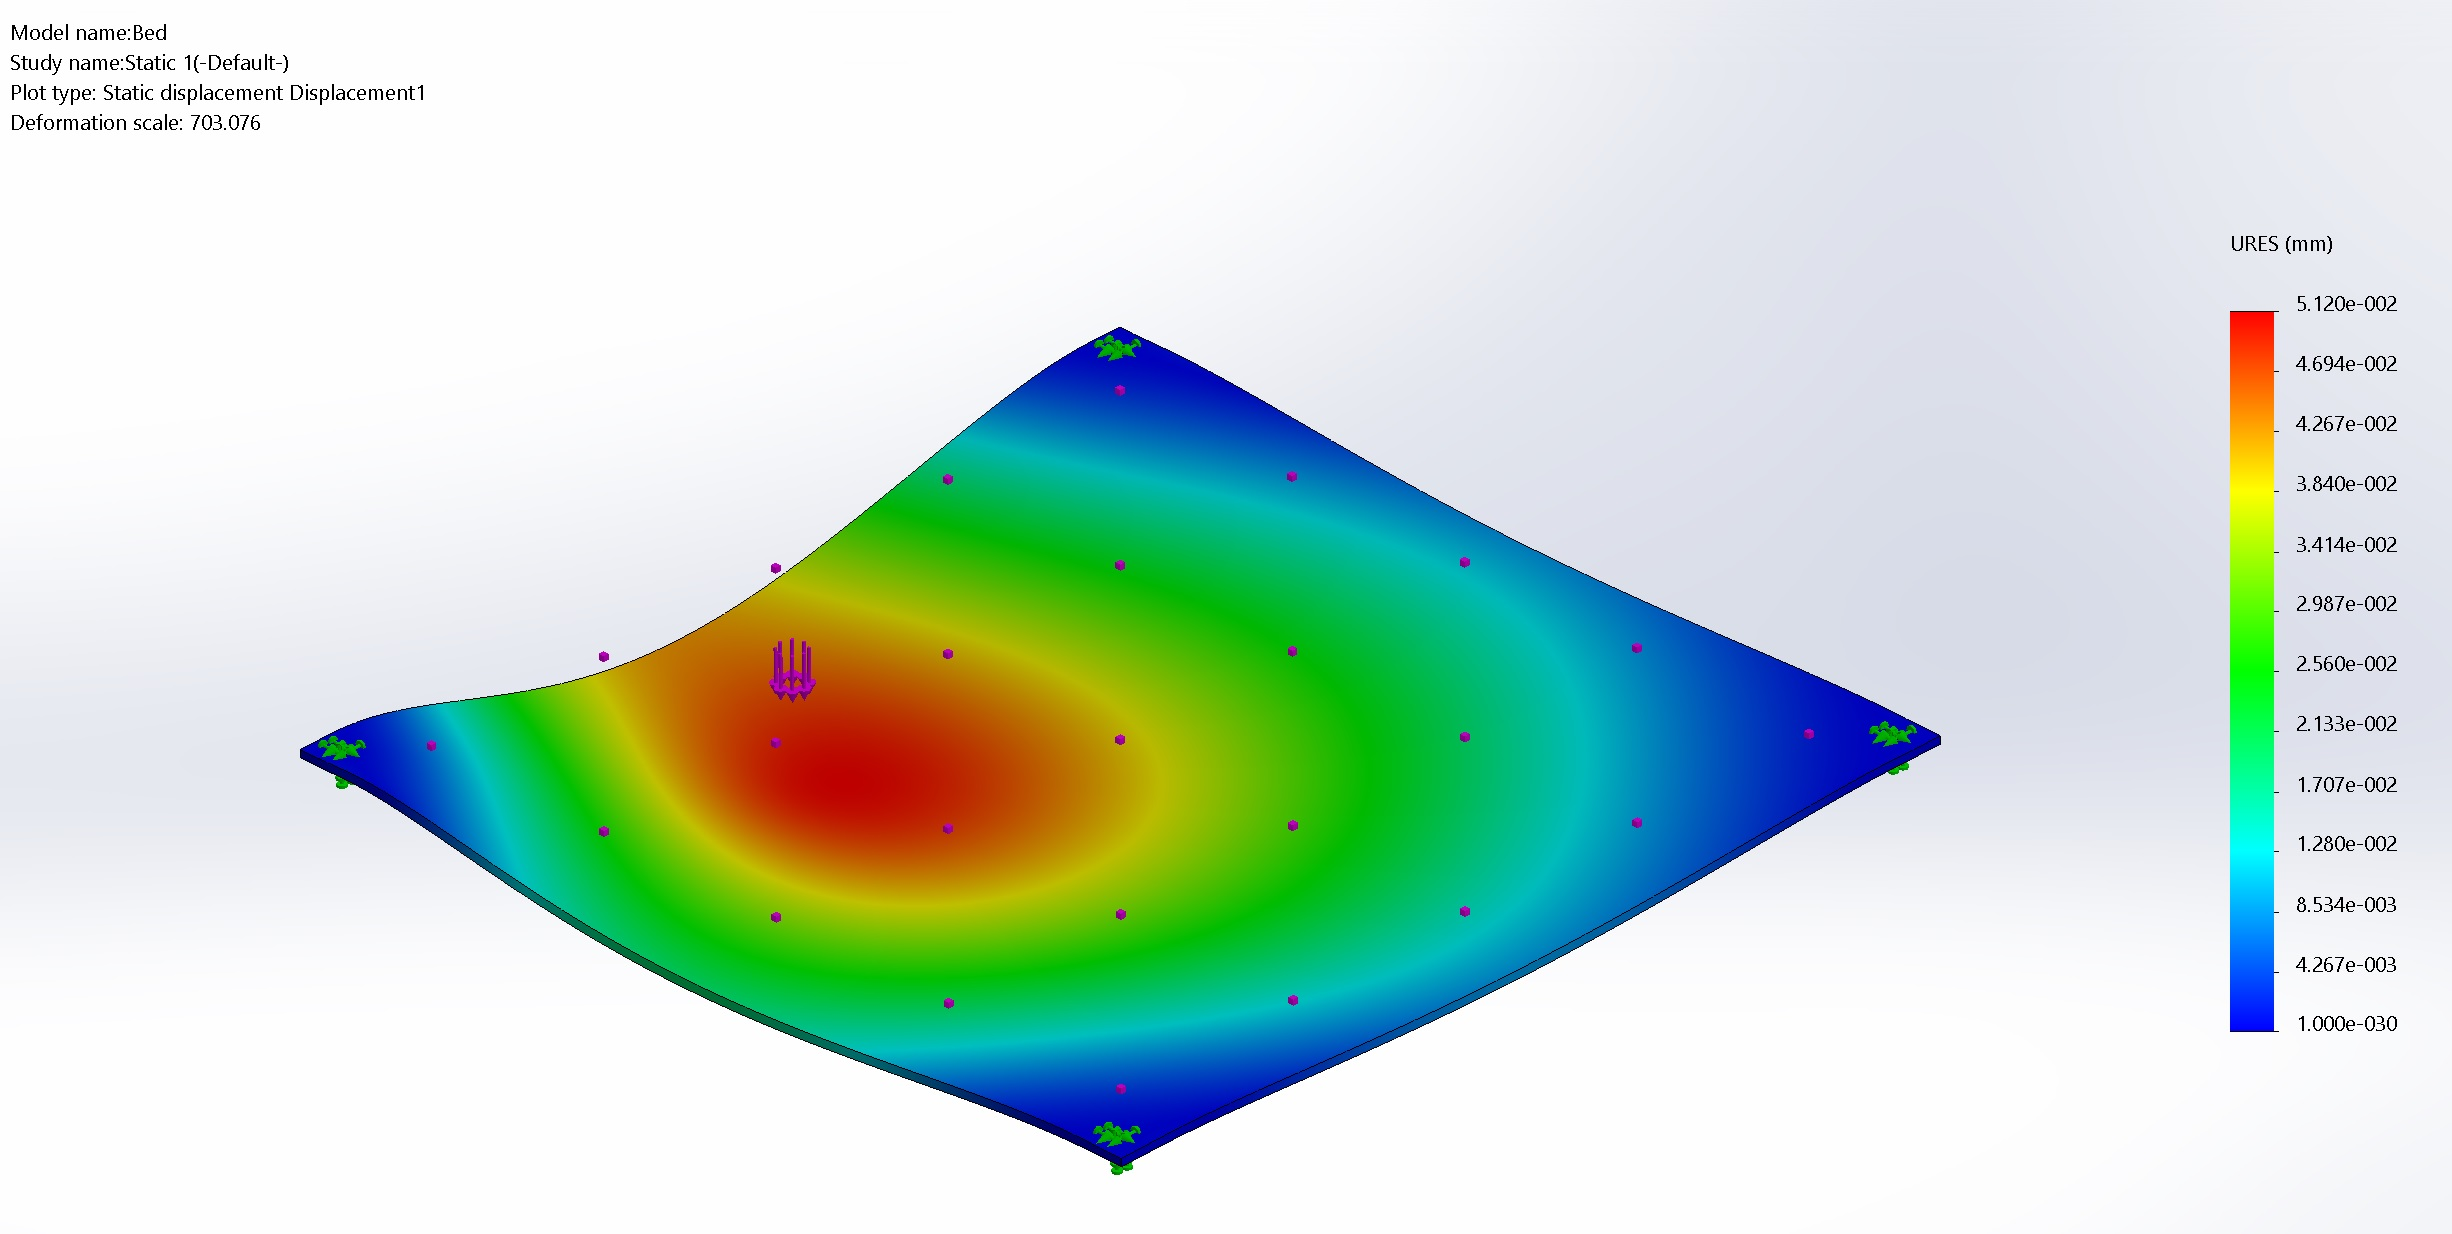
\includegraphics[width=.8\textwidth]{figures/FEM}
			\end{center}
			\caption{FEM static analysis for a hit of 1N in the platform.}
			\label{fig:FEM}
		\end{figure}

		Due to the requirement to make the structure with different positions where allocate the motor, the size of it implies manufacture it with the laser cutting technology. 
		The available let make big parts up to 800 $mm$ so the total structure's height was chosen to be 400, the same has the side of the platform. 
		Based on this size, an $L$ structure was designed to be strong in the X an Y stresses while to absorbs the torque two squads were put in the bottom and the top.
		Also four legs are assemblies in the structure to give more stability and they are the same part has one of the squads so assures easy for big lots.

		The arm is designed to reduce as much as possible the deformation during the movement and when the ball is caught. For manufacture the arm along with the squads, a the FDM technology was used due to the possibilities of the shape it lets and also because of the availability. Finally, the screws and nuts were chosen based on stock. In the figure \ref{fig:render2} a render of the final design is shown.

		\begin{figure}[!hb]
			\begin{center}
				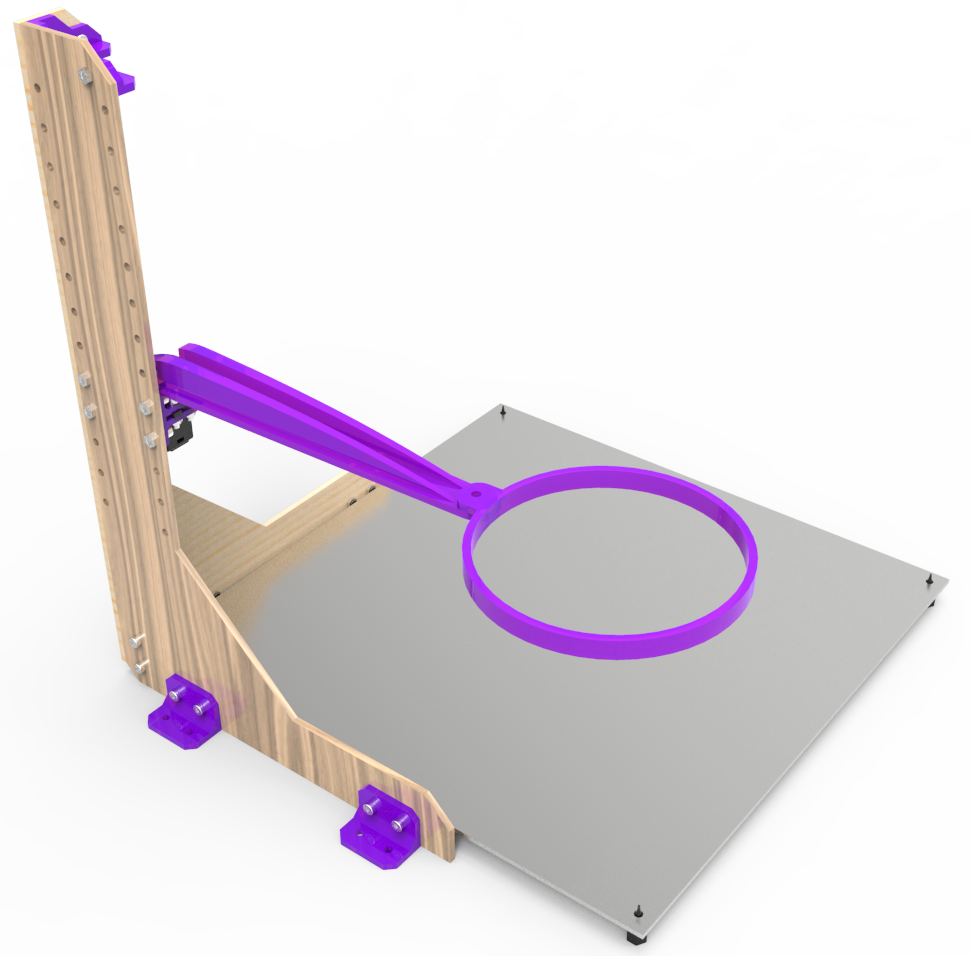
\includegraphics[width=.8\textwidth]{figures/render2}
			\end{center}
			\caption{Render of the final design.}
			\label{fig:render2}
		\end{figure}
	% section manufacturing (end)

	\section{Conclusions} % (fold)
	\label{sec:mechanics_conclusions}
		The assembly of the whole project was as expected and no modifications were required. Some troubles were found while mounting the servo because was kind of difficult to assembly it, but not impossible. That is a point to be improved.

		On the other hand, the structure response as expected and it let carry out all the test necessaries. In the figure \ref{fig:photo1} the final assemble prototype is shown.

		\begin{figure}[tb]
			\begin{center}
				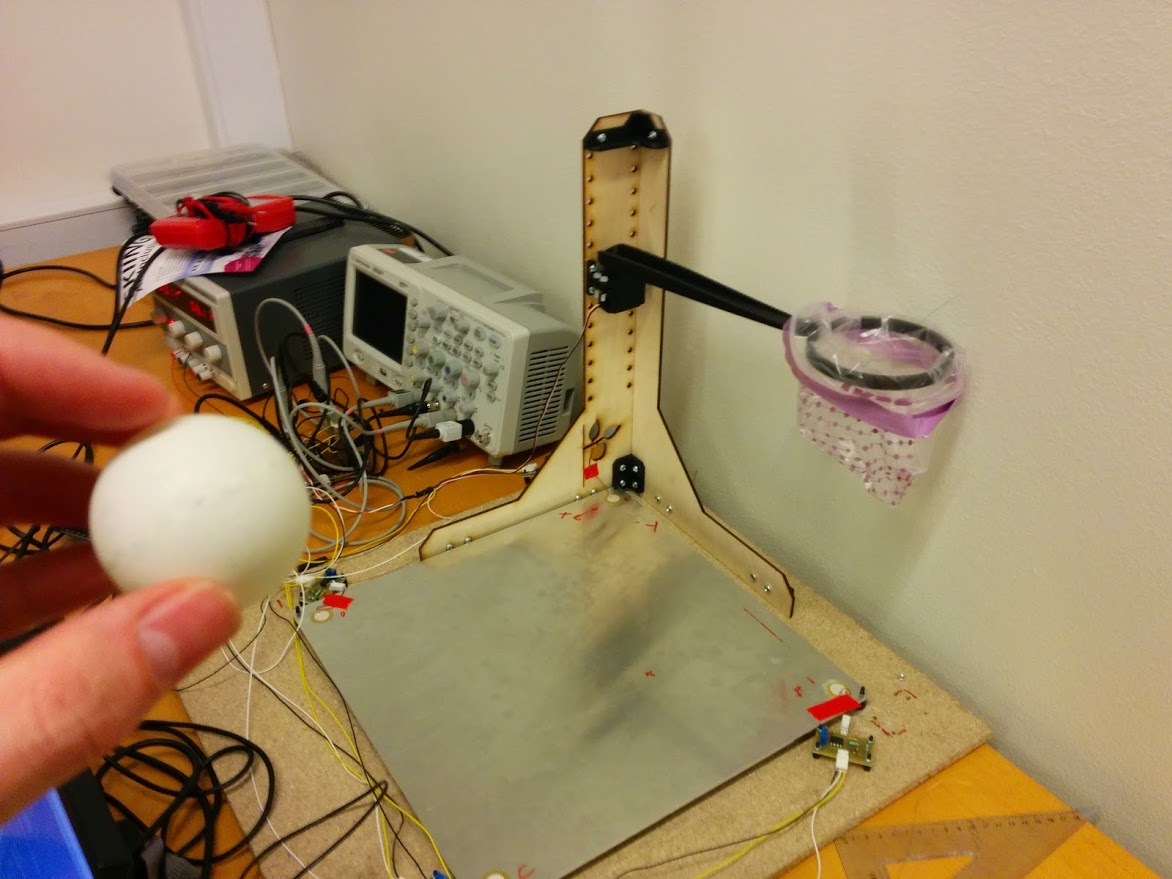
\includegraphics[width=.8\textwidth]{figures/photo1}
			\end{center}
			\caption{Photo of the final assembled prototype.}
			\label{fig:photo1}
		\end{figure}
	% section conclusions (end)
% chapter chapter_name (end)